\subsection{Consulter les menus}

\noindent\textbf{Nom :} Consulter les menus \\
\textbf{ID :} UC102 \\
\textbf{Description :} Le service restauration souhaite pouvoir consulter les menus par groupe de patient. \\
\textbf{Auteur :} Nicolas SYMPHORIEN \\
\textbf{Dates(s) :} 11/06/2017 \\
\textbf{Acteurs :} Le service restauration \\
\textbf{Pré-condition :} L'utilisateur doit être identifié.

\noindent \textbf{Scénario principal :} Figure \ref{ConsulterMenusSeq}

\begin{enumerate}
	\item \label{UC102_step1}Le service restauration choisit le groupe de patient pour lequel il veut voir le menu.
	\item \label{UC102_step2}Le système affiche le menu de la semaine en cours selon le groupe de patient choisi
	\item \label{UC102_step3}Le service restauration peut choisir de consulter le menu pour un autre groupe de patients, dans ce cas le cas d'utilisation reprend à l'étape \ref{UC102_step1}, sinon le cas d'utilisation se termine.
\end{enumerate}

\noindent \textbf{Scénario alternatif :}

\textit{Premier scénario alternatif :}
Le scénario alternatif suivant débute après l'étape \ref{UC102_step2} du scénario nominal
\begin{enumerate}
	\item L'utilisateur peut changer de groupe de patient et le cas d'utilisation reprend à l'étape \ref{UC102_step2} du scénario nominal
\end{enumerate}

\textit{Second scénario alternatif :}
Le scénario alternatif suivant débute après l'étape \ref{UC102_step2} du scénario nominal
\begin{enumerate}
	\item Le service restauration peut changer de semaine
	\item Le système affiche le menu de la semaine choisi s'il existe, sinon il affiche un message. 
\end{enumerate}
Le cas d'utilisation reprend à l'étape \ref{UC102_step3} du scénario nominal.

\noindent \textbf{Post-Conditions:} Le menu est affiché pour le groupe de patients choisi.

\begin{figure}
\centering
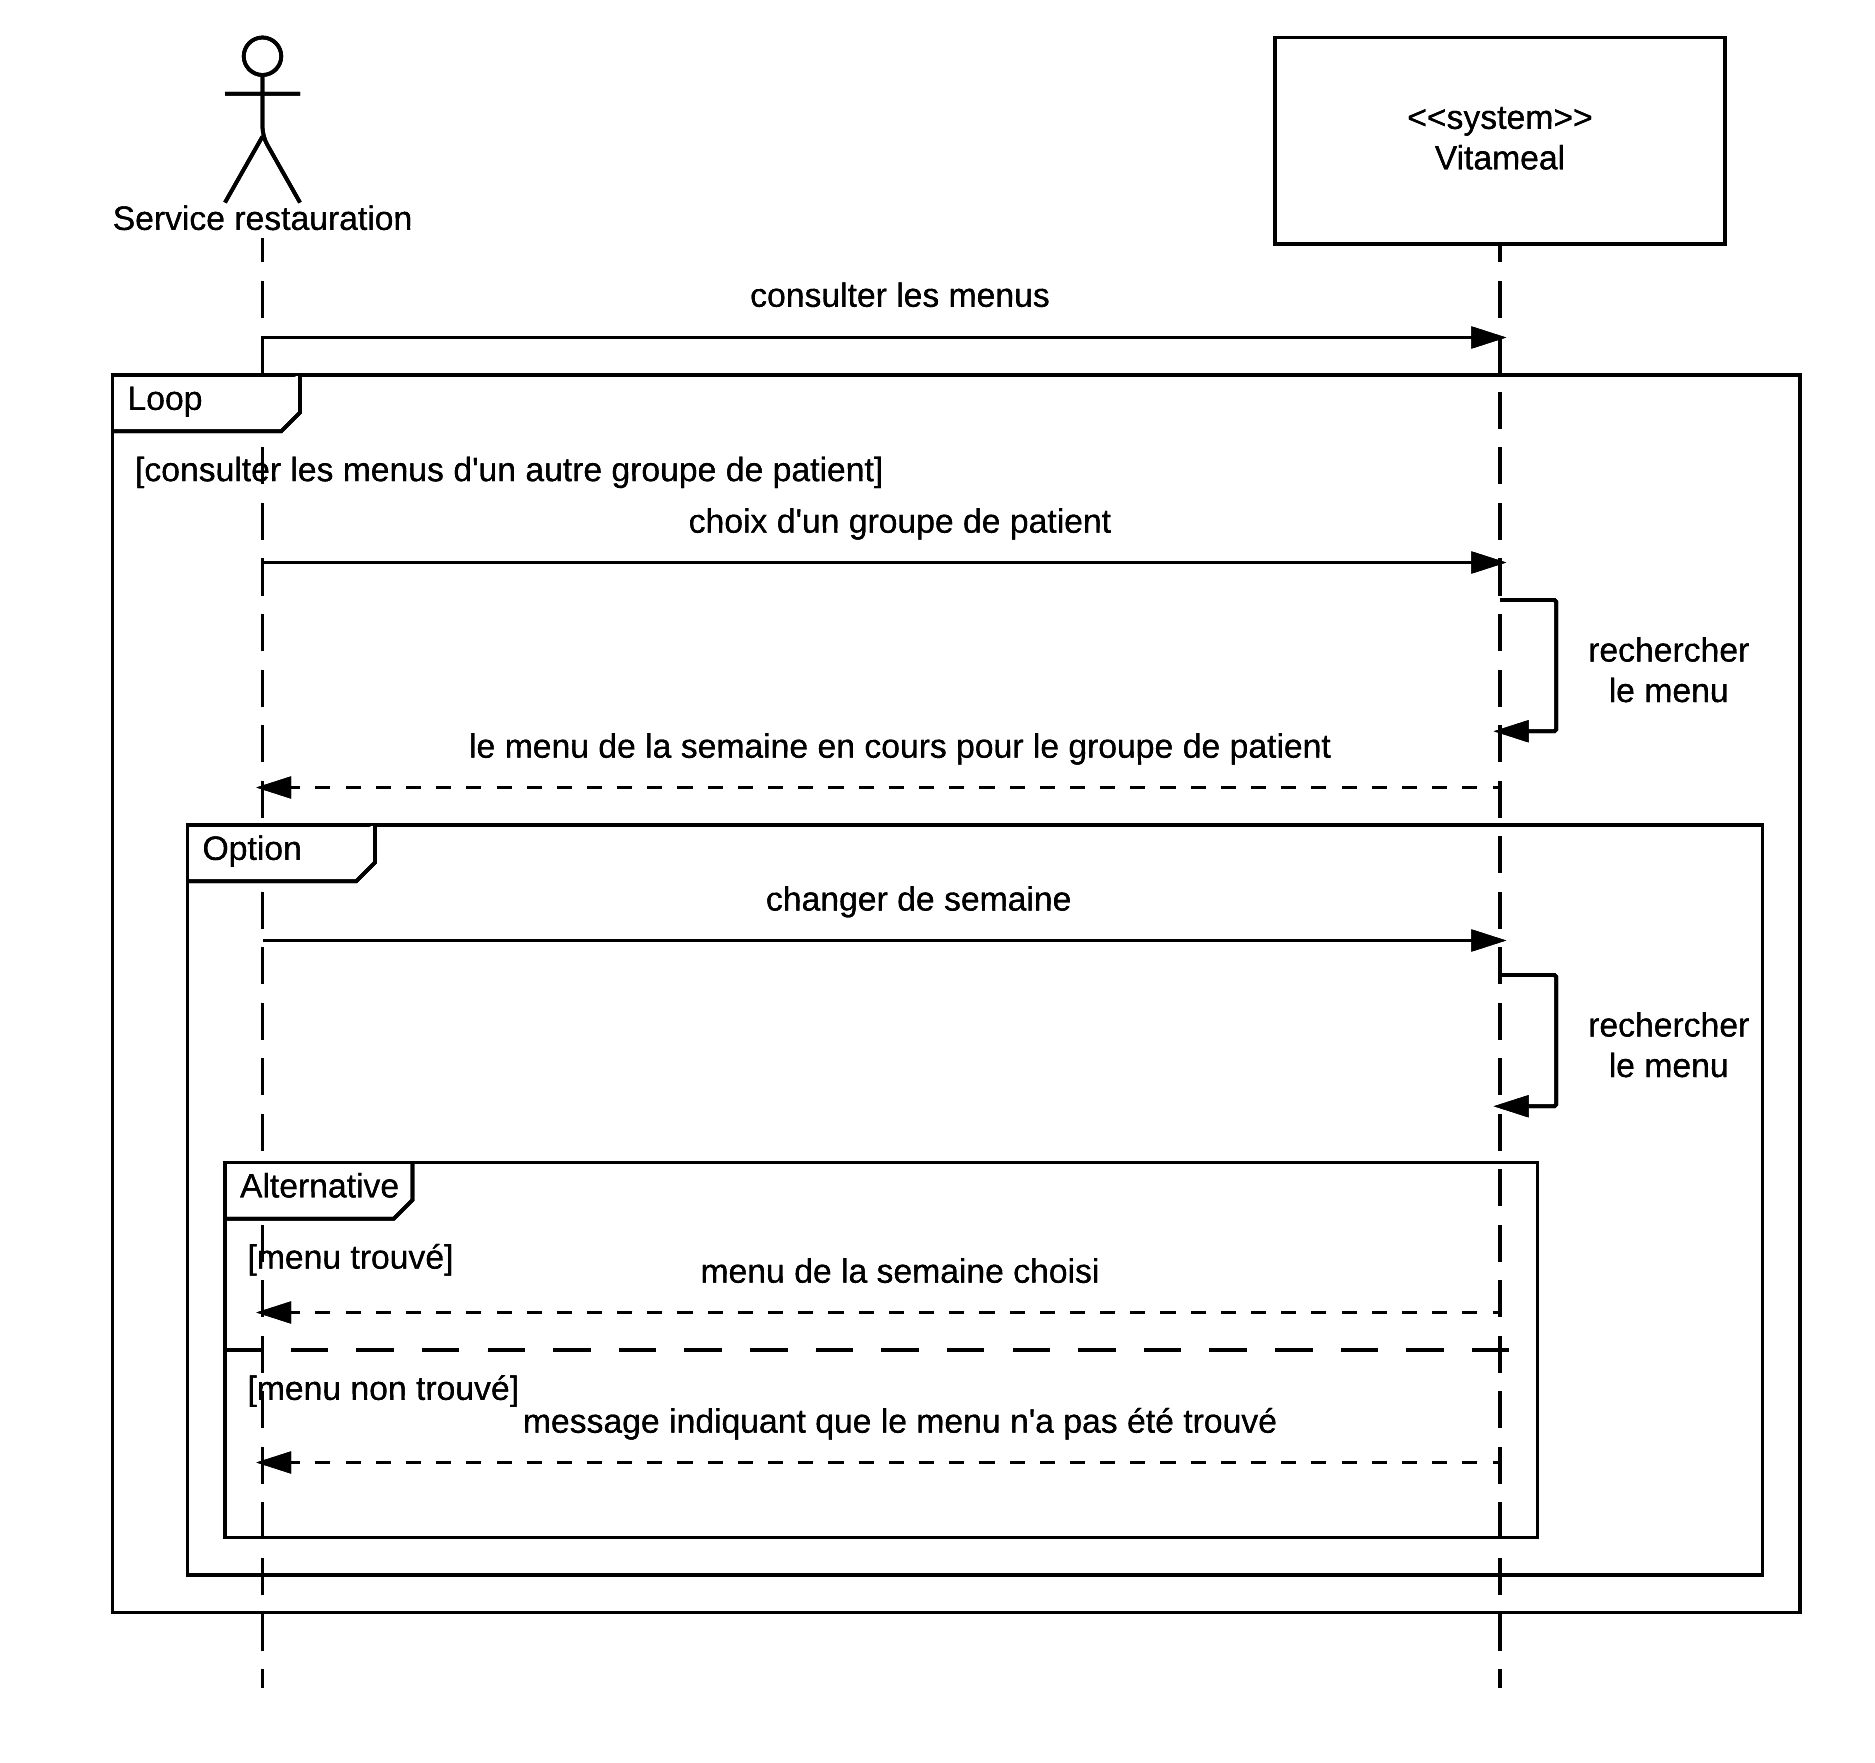
\includegraphics[scale=0.75]{../../CasDUtilisations/ConsulterMenus/sequence_consulter_menus.png}
\caption{Diagramme de séquence du cas d'utilisation consulter les menus}
\label{ConsulterMenusSeq}
\end{figure}
